\section{Beyond graphene: TMD nanoribbons}
\label{sec:state}

\ac{2D} materials have steadily been drawing the attention of the community since graphene was experimentally isolated from a graphite sample by mechanical exfoliation, yielding a system constituted by a single layer of atoms (Fig. (\ref{fig:graphene}), left).
Since then, numerous studies have been made due to the promising properties of these materials, and the interesting as-yet-unseen phenomena occurring within them, for example, in the case of graphene: unconventional quantum Hall effect, absence of localization, and electrons behaving like massless relativistic particles near the $K$ points, where the dispersion relation is approximately linear (Fig. (\ref{fig:graphene}), right), providing a bridge between condensed matter physics and quantum electrodynamics \cite{katsnelson_graphene:_2007}.
In spite of its undeniable potential, graphene has some shortcomings.
This motivated the community to study other more complex graphene-like materials, which could have other desirable properties, while maintaining most of graphene's potential.

\begin{figure}[H]
\hspace{1.5cm}
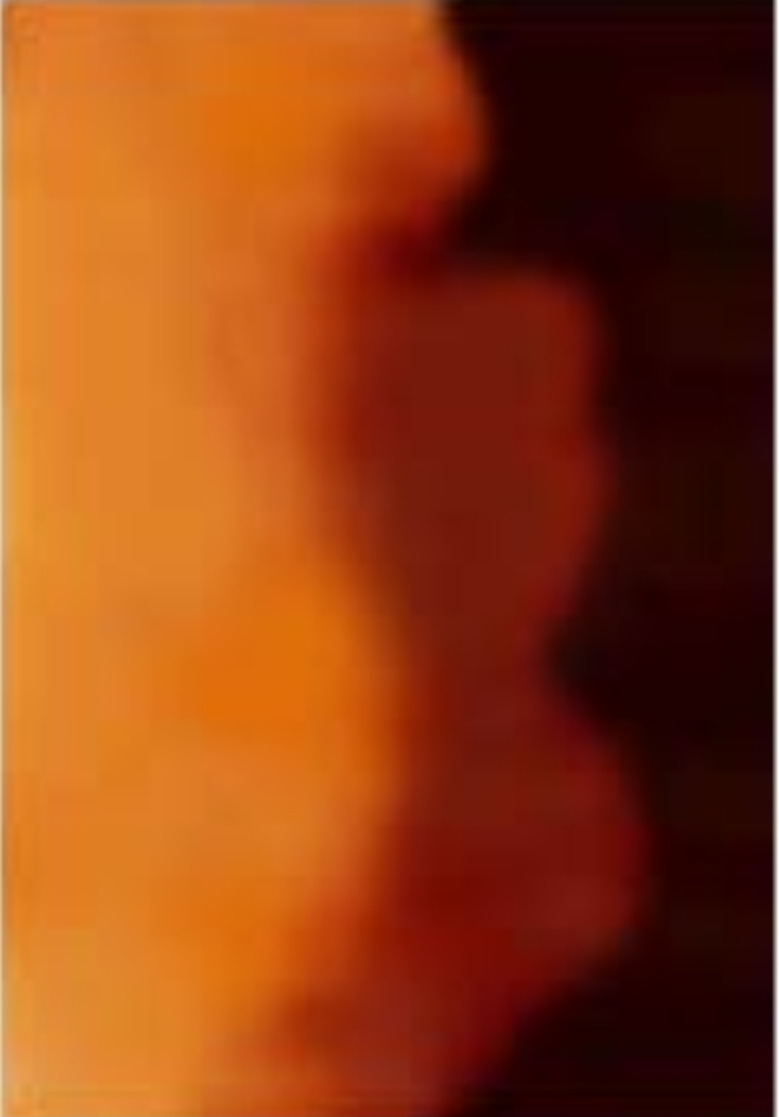
\includegraphics[width = 3.2cm]{Introduction/graphene.png}
\hspace{2cm}
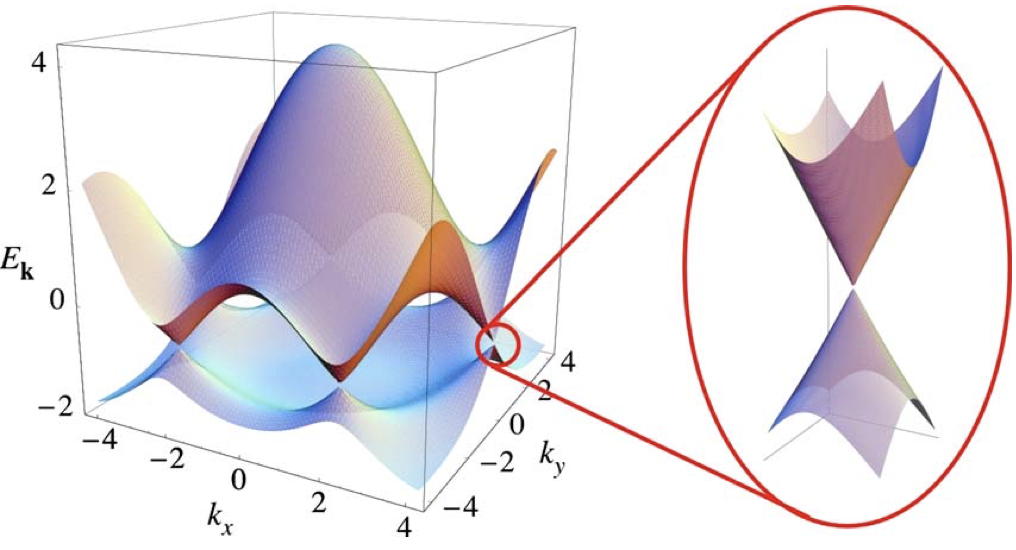
\includegraphics[width = 8cm]{Introduction/dispGraphene.png}
\caption[Graphene monolayer; graphene's dispersion relation.]{Left: \acf{AFM} picture of a graphene monolayer. The black area is a substrate used for fabrication purposes. The dark orange area is a monolayer of graphene. Right: Dispersion relation of graphene. The Fermi energy is set to zero. Close to it, the dispersion relation is linear, corresponding to massless excitations (taken from \cite{castro_neto_electronic_2009}). }
\label{fig:graphene}
\end{figure}	

\acp{TMD} are prominent examples of such novel members of the \ac{2D} materials family \cite{wang_electronics_2012, roldan_electronic_2014, xu_spin_2014}.
An excellent review of their properties, experimental results and applications is given in \cite{manzeli_2d_2017}.
Much like graphite which is essentially constituted by stacked monolayers of carbon atoms bound by weak Van der Waals forces, 3D \ac{TMD} structures are also formed by weakly bound layers.
However, instead of carbon, the layers contain transition metals $M$, and chalcogens $X$, in a two $X$ to one $M$ proportion.
Thus, group 6 \acp{TMD} are denoted $MX_2$, where $M = \text{Mo}, \text{W}, ...$ (respectively Molybdenum and Tungsten) and $X = \text{S}, \text{Se}, \text{Te}$ (respectively Sulfur, Selenium and Tellurium).
Each monolayer contains a layer of $M$ atoms organized in a triangular lattice sandwiched between two layers of $X$ atoms, as opposed to graphene, where carbon atoms are all on the same plane.
Each $M$ atom is coordinated with six $X$ atoms, giving rise to a stacked structure with various possible coordinations, depending on the spatial arrangement of the $X$ atoms.
The most common structural phases are trigonal prismatic (2H) and octahedral (1T).
\ac{TMD} monolayers are still considered \ac{2D} since their thickness is at the atomic scale.
For example, for molybdenum disulfide, $\text{Mo} \text{S}_2$, monolayers are only $ 6.5 \angstrom$ thick.
For this reason, for the particular case of the 2H phase we shall focus on from now on, the $M-X$ lattice is thought of as being hexagonal, as seen in the top-down view of Fig (\ref{fig:tmdHex}a).
Valence bands arise out of the hybridization of the $d_{xy}$ and $d_{x^2 - y^2}$ orbitals of the transition metal and the $p_{x, y}$ orbitals of the chalcogen, while conduction bands have a main contribution from the $d_{3z^2 - r^2}$ orbitals of the $M$ atoms with only a minor contribution from the $p_{x, y}$ orbitals of the $X$ atoms.

\begin{figure}[H]
\centering
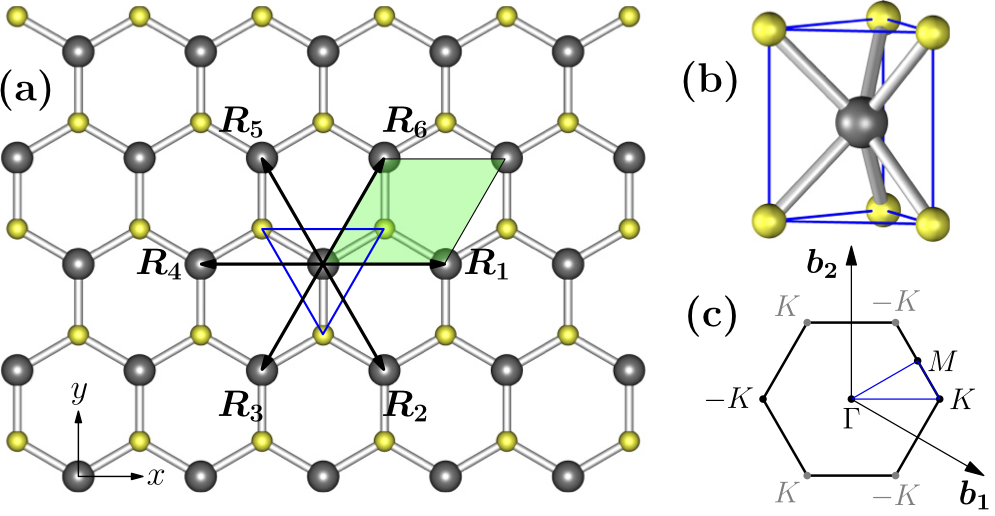
\includegraphics[scale = 0.25]{Introduction/tmd2.png}
 \caption[\ac{TMD} monolayer condensing in its 2H phase.
 $M-X$ honeycomb lattice.
 Unit cell of the trigonal prismatic (2H) phase of a \ac{TMD} monolayer.
 High symmetry points of the corresponding hexagonal lattice's  reciprocal space.]{(a) The 2H phase of a  \ac{TMD} monolayer may be viewed simply as a $M-X$ honeycomb lattice. Here we represent the six nearest neighbors of a point on the $M$ triangular lattice by the real space vectors $\bm R_{i = 1,2,..., 6}$.
(b) Unit cell of the trigonal prismatic (2H) phase of a \ac{TMD} monolayer.
(c) High symmetry points $\Gamma, M, K$ of the first Brillouin zone ($\bm b_{1,2}$ are the reciprocal basis vectors).\label{fig:tmdHex}}
\end{figure}

\ac{2D} \acp{TMD} have been attracting interest because they seem to overcome some of the drawbacks of graphene in technological applications.
For example, monolayer graphene is gapless, while its bilayer counterpart has a tunable, but small gap of the order of a tenth of an $eV$.
Contrastingly, monolayer \acp{TMD} have an intrinsic gap in excess of $1 \, eV$, lying at the inequivalent $K$ points of the hexagonal Brillouin zone, being more promising in designing, for example, transistors.
Hole-doped \acp{TMD} are expected to show topological superconductivity \cite{hsu_topological_2017}, while the superconducting phase of graphene has been predicted, but is not easily attained.
Superconductivity in graphene-like \ac{2D} materials is important because it could boost high speed nanoelectronics.
Moreover, the presence of transition metal atoms in \acp{TMD} suggests the possibility of magnetic ordering \cite{braz_valley_2017}, which could be very relevant in nanospintronics applications.
Both superconductivity and magnetic ordering may arise due to the effect of strong electron correlations.
Thus, to investigate these properties of \acp{TMD} reliably, we need a computational method that is robust enough to capture the effects of strong electron interactions accurately.
As we shall see, auxiliary field \ac{QMC}  fulfills this criterion.

\subsection{Electronic properties}\label{subsec:electronic}

The electronic properties of \ac{TMD} monolayers depend crucially on the coordination.
In particular, for the 2H phase, they may ultimately be attributed to the lack of inversion symmetry relative to the $M$ atoms.
This leads to spin splitting of the electronic bands driven by spin-orbit coupling.
Because $K$ and $K'$ (or $-K$) no longer correspond to time reversal invariant momenta, the spin degeneracy of the valence and conduction bands is lifted at these points.
Time reversal symmetry implies that the splitting is opposite at the $K$ and $K'$ points, leading to the band structure of Fig. (\ref{fig:tmdProp}d) (we show the part relevant for realistic charge-carrier concentrations).
This property, known as spin-valley coupling, implies that the valley polarization of charge carriers directly translates into spin polarization, leading to an intrinsic property of \acp{TMD} that could allow one to design spintronic devices without resorting to magnetic materials \cite{manzeli_2d_2017}.
More broadly, the possibilities afforded by the different compositions and structural phases listed in Fig.(\ref{fig:tmdProp}) lead to a vast array of electronic properties.
On the one hand, the band structure and its metallic/insulating character vary quite substantially among \acp{TMD}.
On the other hand, both highly nontrivial  correlated and topological phases arise within these materials.
In this work, we investigate the properties of correlated phases in zigzag edged \ac{TMD} nanoribbons.

\begin{figure}[H]
\centering
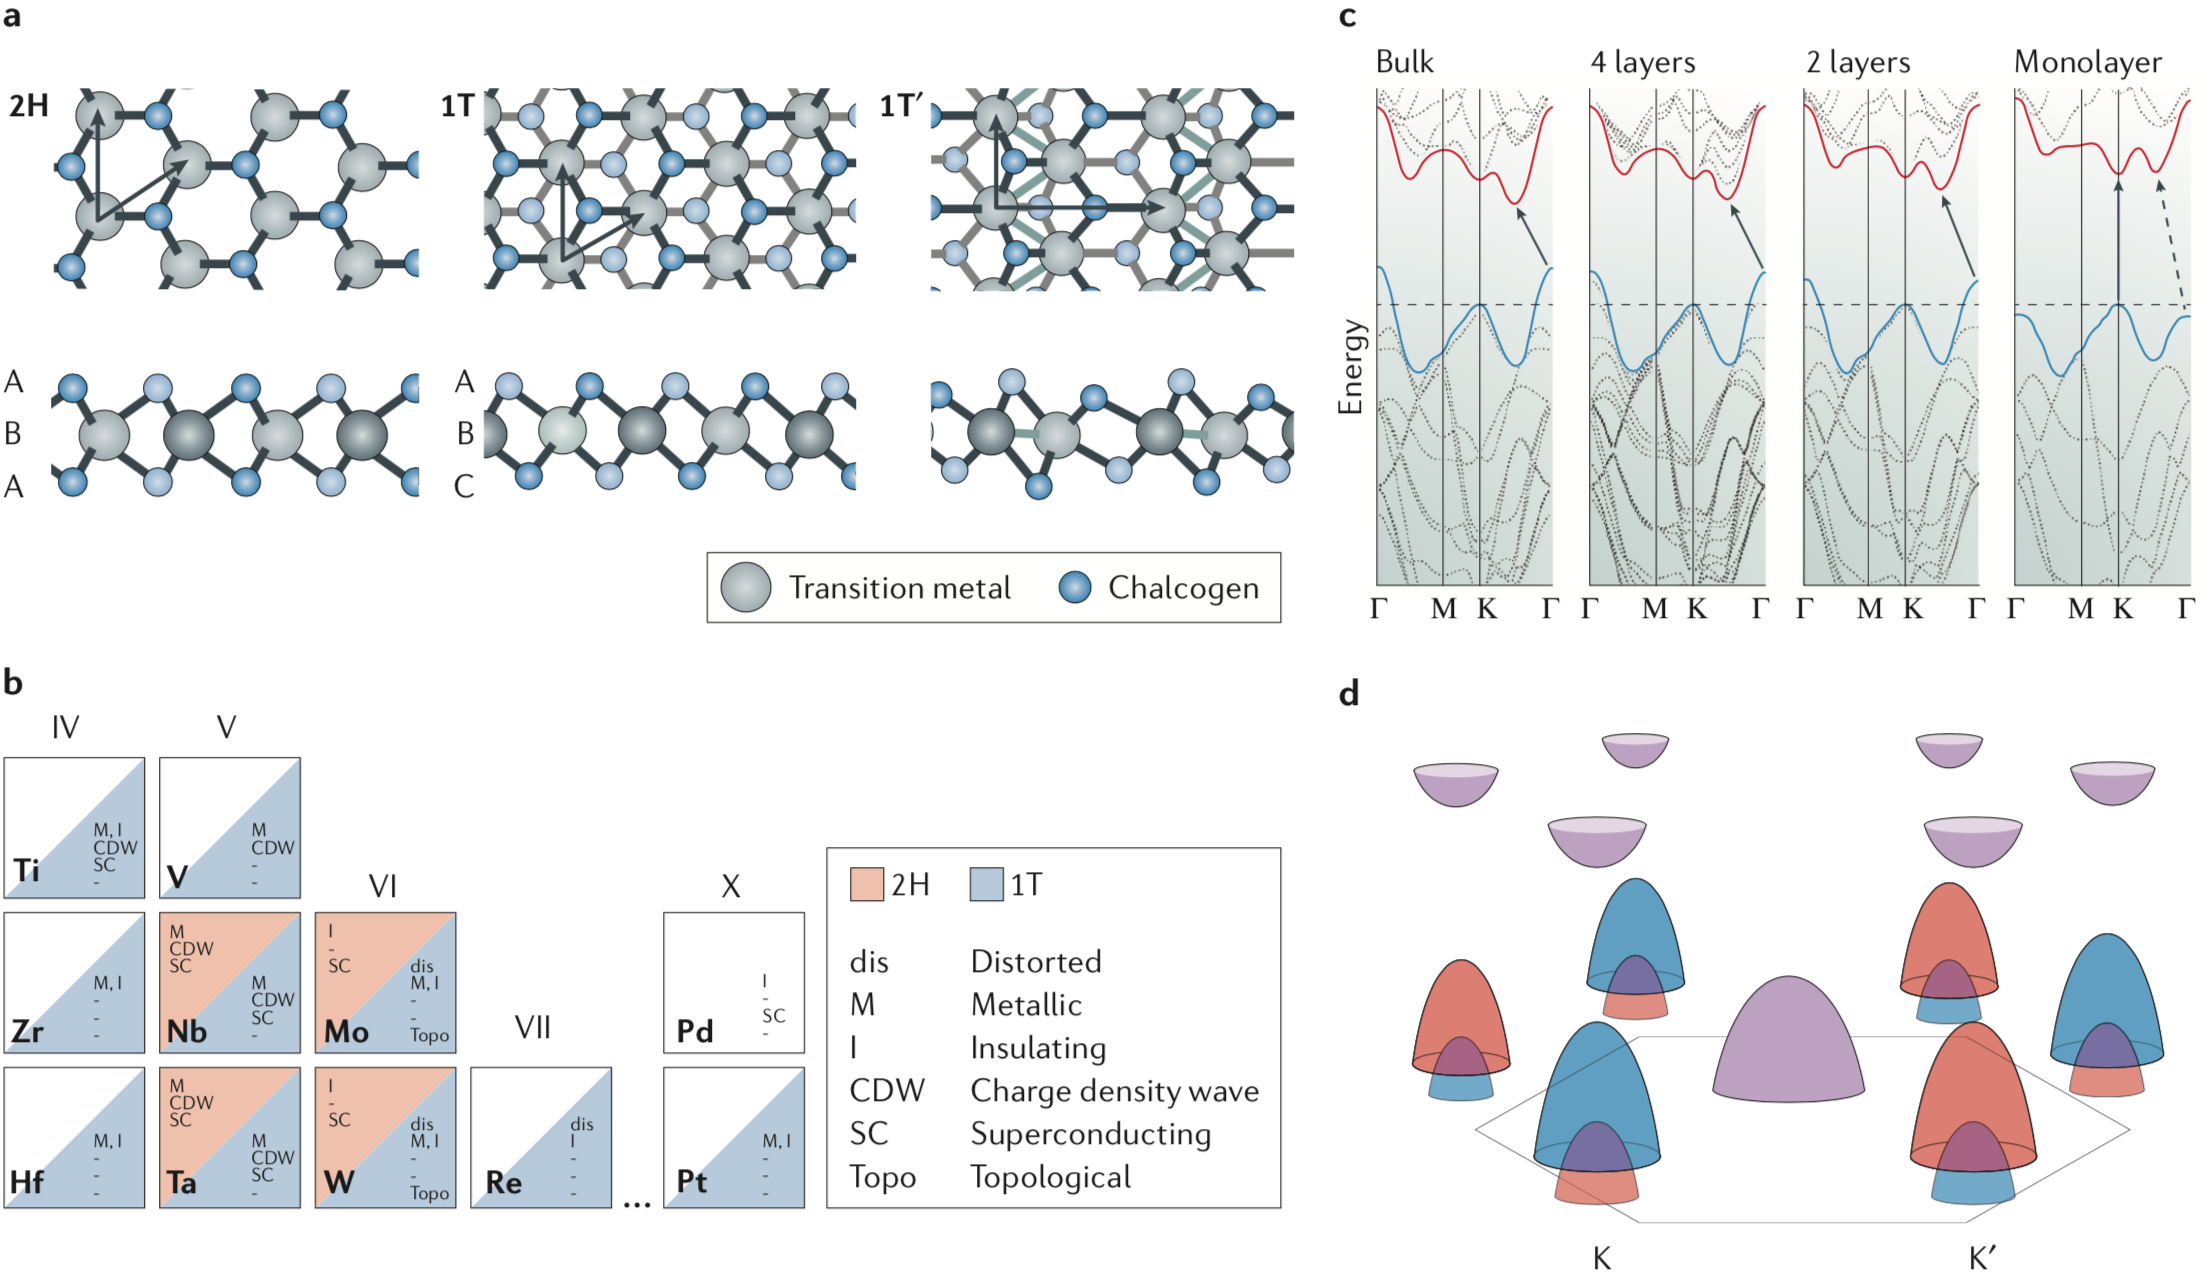
\includegraphics[scale = 0.35]{Introduction/tmdProp}
 \caption[Structure and electronic properties of \ac{TMD} monolayers.]{(a) Examples of some of the possible structural phases of \ac{TMD} monolayers: trigonal prismatic (2H) with ABA stacking, distorted octahedral (1T), and dimerized octahedral (1T'), showing ABC stacking. (b) A periodic table of known \ac{TMD} layers. Shown are the transition metals involved, the existing phases (2H and/or 1T), and the possible electronic phases. (c) Calculated band structure (from density functional theory \cite{splendiani_emerging_2010} ) of $2H-\text{Mo}\text{S}_2$ for samples of decreasing thickness. (d) Representation of the band structure of monolayer $2H-\text{Mo}\text{S}_2$, showing the spin splitting (red for spin-up and blue for spin-down) of the bands near the corners of the Brillouin zone (K and K') points. \label{fig:tmdProp}}
\end{figure}

\subsection{Nanoribbons}\label{subsec:nanoribbons}

Nanoribbons are a particularly promising type of \acs{2D} nanostructure.
A nanoribbon consists of a \ac{2D} layer that can be regarded as infinitely long on one direction, but not on the other (Figs. (\ref{fig:fabrication}) and (\ref{fig:graphNano})), so that edge states become relevant, and can be controlled to yield interesting properties.
For simulation purposes, it is natural to assume translational invariance along the ribbon's longitudinal direction, and use \acp{PBC}.
On the other direction, we use \acp{OBC}, effectively considering zigzag edges (see Fig.(\ref{fig:nanoribbons}), left).

\begin{figure}[H]
\centering
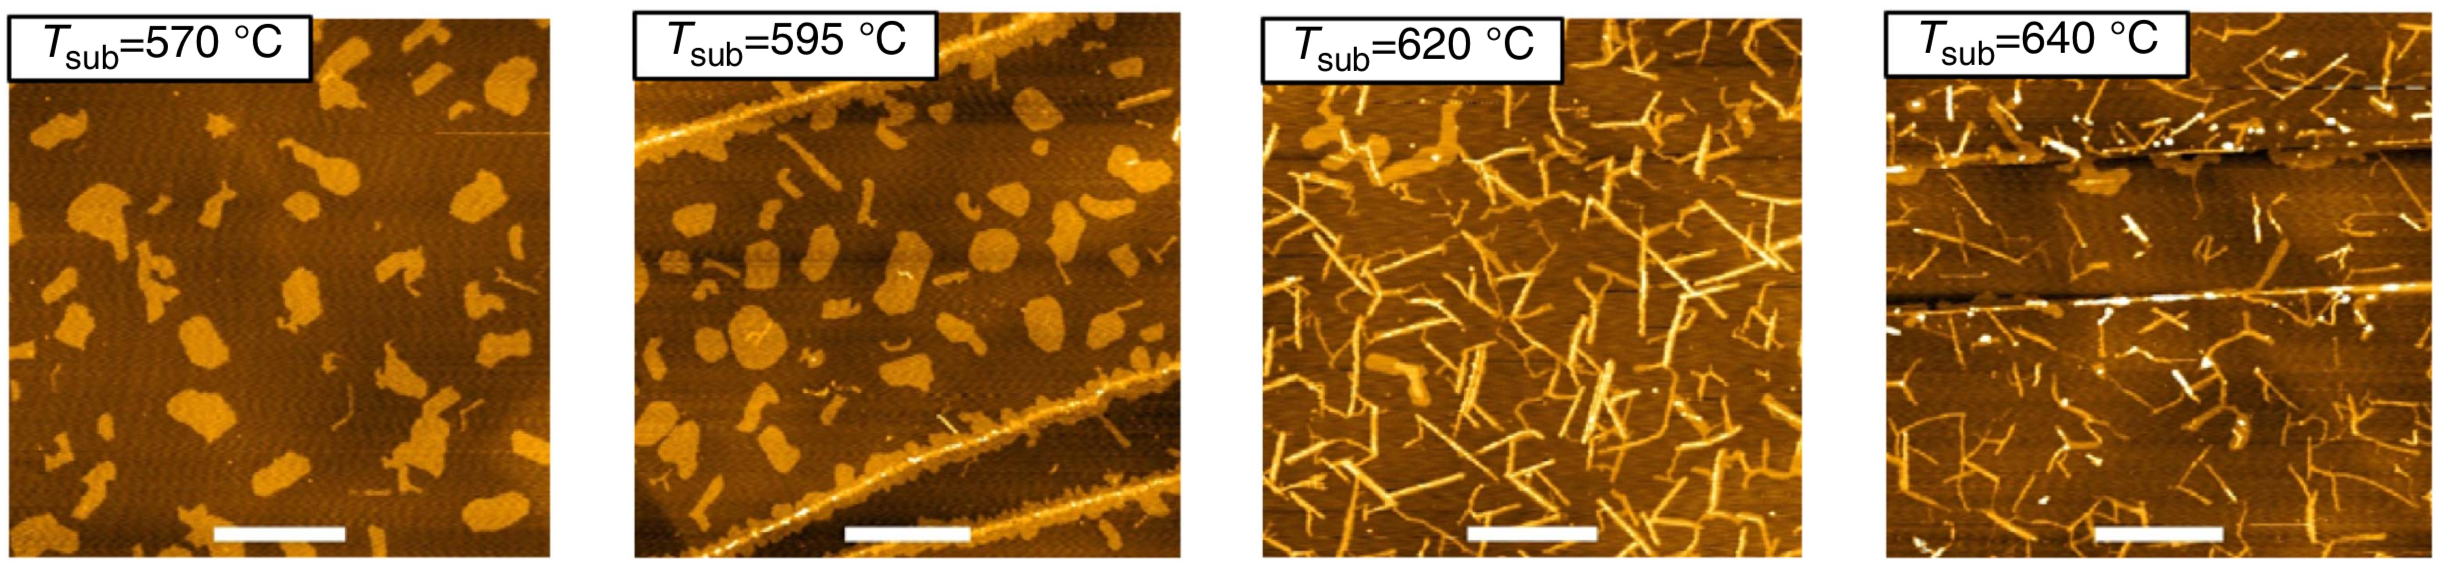
\includegraphics[scale = 0.35]{Introduction/nanoribbons}
\caption[Fabrication of \ac{TMD} nanoribbons]{Fabrication of \ac{TMD} nanoribbons. From left to right, we see \ac{AFM} images showing the appeareance of nanostructures ranging from \ac{2D} nanoislands to nanoribbons, as the temperature of the substrate is increased. The nanoribbons are grown by taking advantage of the temperature dependence of shape transformations occuring during the nonequilibrium growth of surface-based nanostructures (taken from \cite{chen_fabrication_2017}).}
\label{fig:fabrication}
\end{figure}

\begin{figure}[H]
\vspace{-0.5cm}
\centering
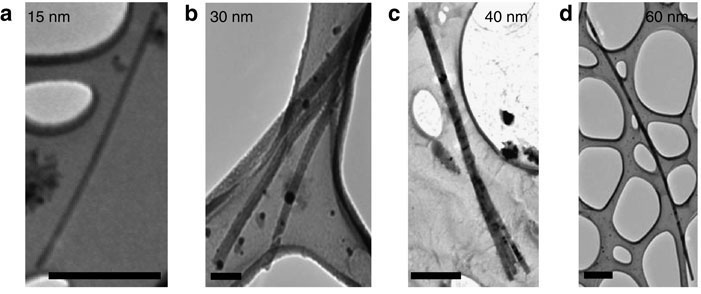
\includegraphics[scale = 0.42]{Introduction/grapheneNanoribbons.jpg}
\caption[(TEM) images of graphene nanoribbons.]{(a) to (d) - Transmission electron microscopy (TEM) images of graphene nanoribbons (GNRs) of widths 15, 30, 40, and 60 $nm$, respectively (adapted from \cite{mohanty_nanotomy-based_2012}).}
\label{fig:graphNano}
\end{figure}
   
A high density of low-energy electronic states is localized at the zigzag edges, decaying quickly in the bulk, which suggests the possibility of magnetic ordering.
In fact, a mean field solution of the Hubbard model for a graphene nanoribbon shows that magnetic moments are localized at the edges \cite{yazyev_emergence_2010} (see Fig.(\ref{fig:nanoribbons}), right).
QMC has been used to investigate edge-state magnetism beyond mean field in graphene \cite{feldner_dynamical_2011, golor_quantum_2013, cheng_strain-induced_2015, raczkowski_interplay_2017, yang_strain-tuning_2017}.
However, edge-state magnetism in \acp{TMD} remains unexplored \cite{davelou_nanoribbon_2017}, and we would like to investigate, for example, whether edge-state magnetism is stabilized at finite temperature in \acp{TMDNR}, following the tendency that was identified for their graphene counterparts.

While the zigzag graphene nanoribbon antiferromagnetic ground state is semiconducting, a state with interedge ferromagnetic orientation is a metal.
An example of an application based on the switching between the two states is a magnetorresistive sensor.
This device allows switching between low and high-resistance configurations, corresponding, respectively, to parallel, and antiparallel configurations of ferromagnetic leads at the ends of a nanoribbon.
An analogous form of edge-state magnetism, as is observed in graphene nanoribbons, for \acp{TMDNR}, could yield similarly innovative applications.

\begin{figure}[H]
\vspace{-0.5cm}
\hspace{0.5cm}
\begin{minipage}[c]{0.1\textwidth}
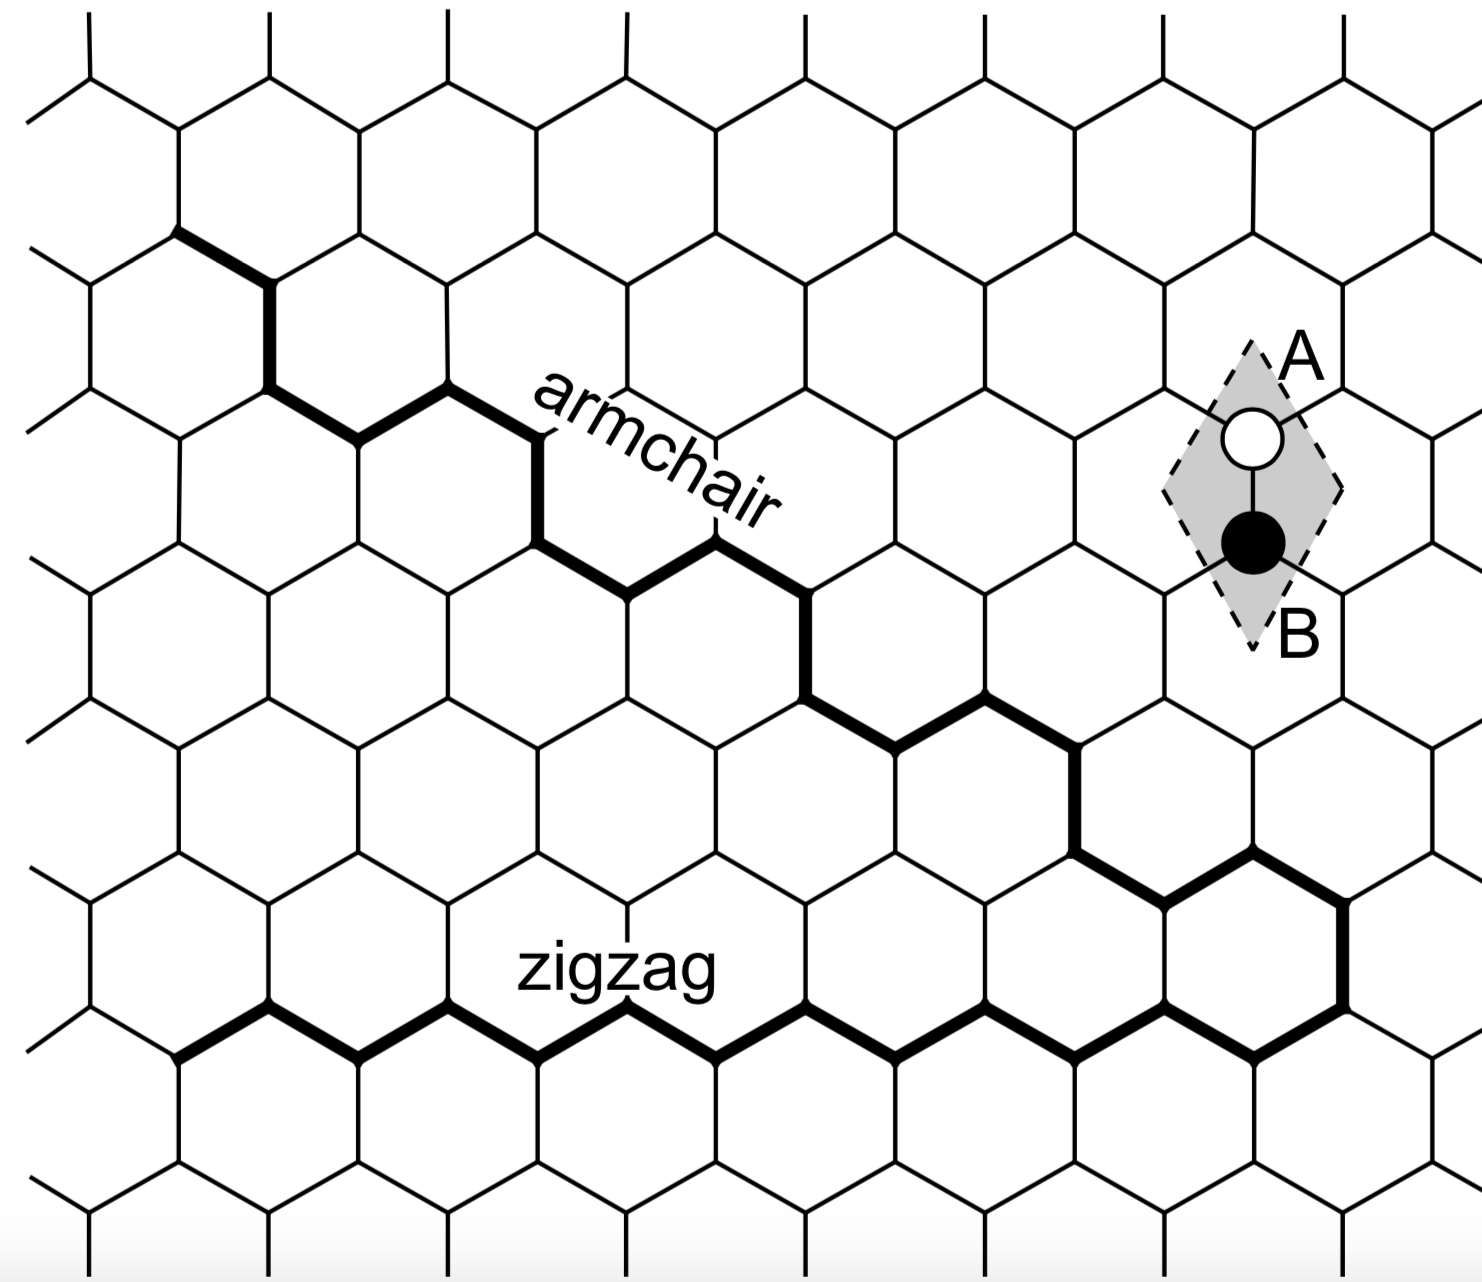
\includegraphics[scale = 0.21]{Introduction/zigzag}
\end{minipage} \hspace{4.2cm}
\begin{minipage}[c]{0.1\textwidth}
\vspace{0.3cm}
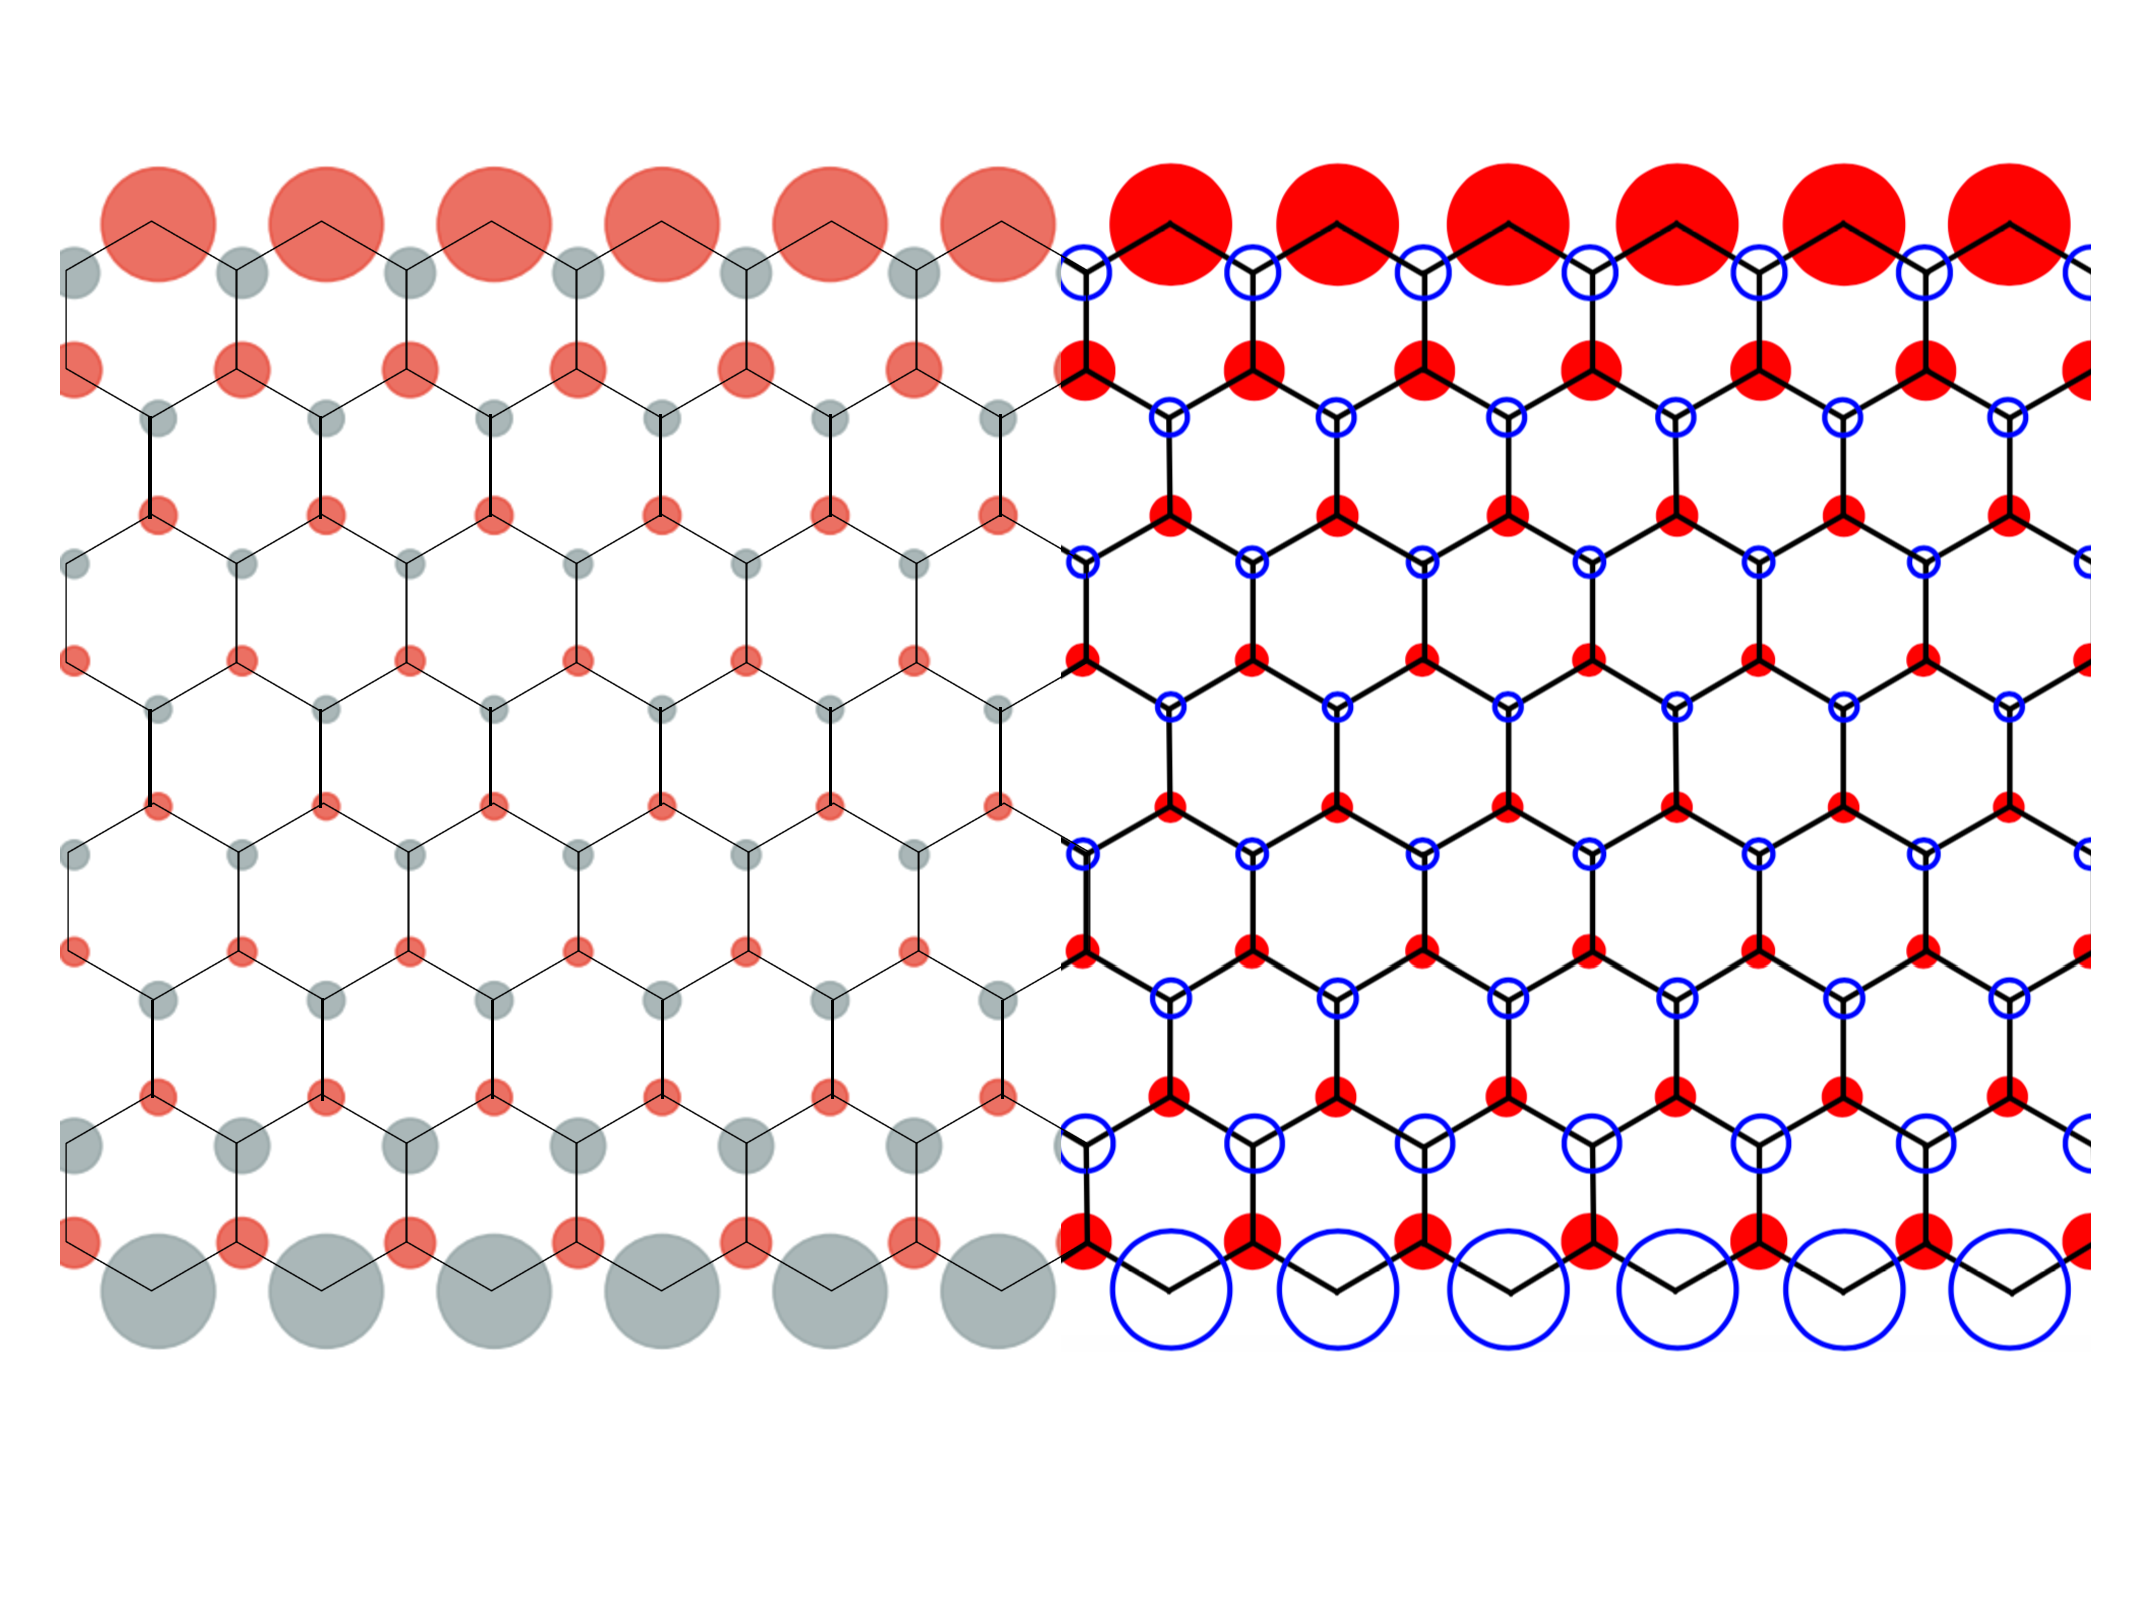
\includegraphics[scale = 0.24]{Introduction/comparisonMF.pdf}
\end{minipage}
\vspace{-0.5cm}
 \caption[Zigzag edges of a nanoribbon and magnetism.]{Left: Two possible terminations of a \ac{TMD} nanoribbon condensing in a honeycomb lattice.
Right: Example of a mean field result for a  graphene nanoribbon.
Local magnetic moments tend to develop significantly on zig zag edges.
The area of the circles corresponds to the magnitude of the magnetic moment.
The red circles corresponds to the spin up density, and the blue ones to the spin down density.
The particular arrangement of the electronic edge states leads to an \ac{AF} ground state (opposite edges with opposite magnetic moment). The results on the right part of the picture are taken from \cite{yazyev_emergence_2010}, while the left part corresponds to our original results clearly reproducing the ones on the literature). \label{fig:nanoribbons}}
\end{figure}

\subsection{Effective three-band minimal tight-binding model}\label{subsec:threeband}

In this section, we present a minimal model describing the low energy physics of group 6 \acs{TMD} monolayers \cite{liu_three-band_2013}.
To obtain this tight-binding model, one uses the symmetries of the monolayers, and the fact that conduction and valence band edges have major contributions from $d_{z^2}$, $d_{xy}$, and $d_{x^2 - y^2}$ orbitals of $M$-atoms.
This is illustrated for $\text{Mo}\text{S}_2$ in Fig.(\ref{fig:energiesTMDs}).
Near the Fermi energy, the $\text{Mo}$ $d$-orbitals are clearly more populated at the $K$ point (circled in orange), hence these states contribute more to the energy dispersion near the $K$ points.

\begin{figure}[H]
\centering
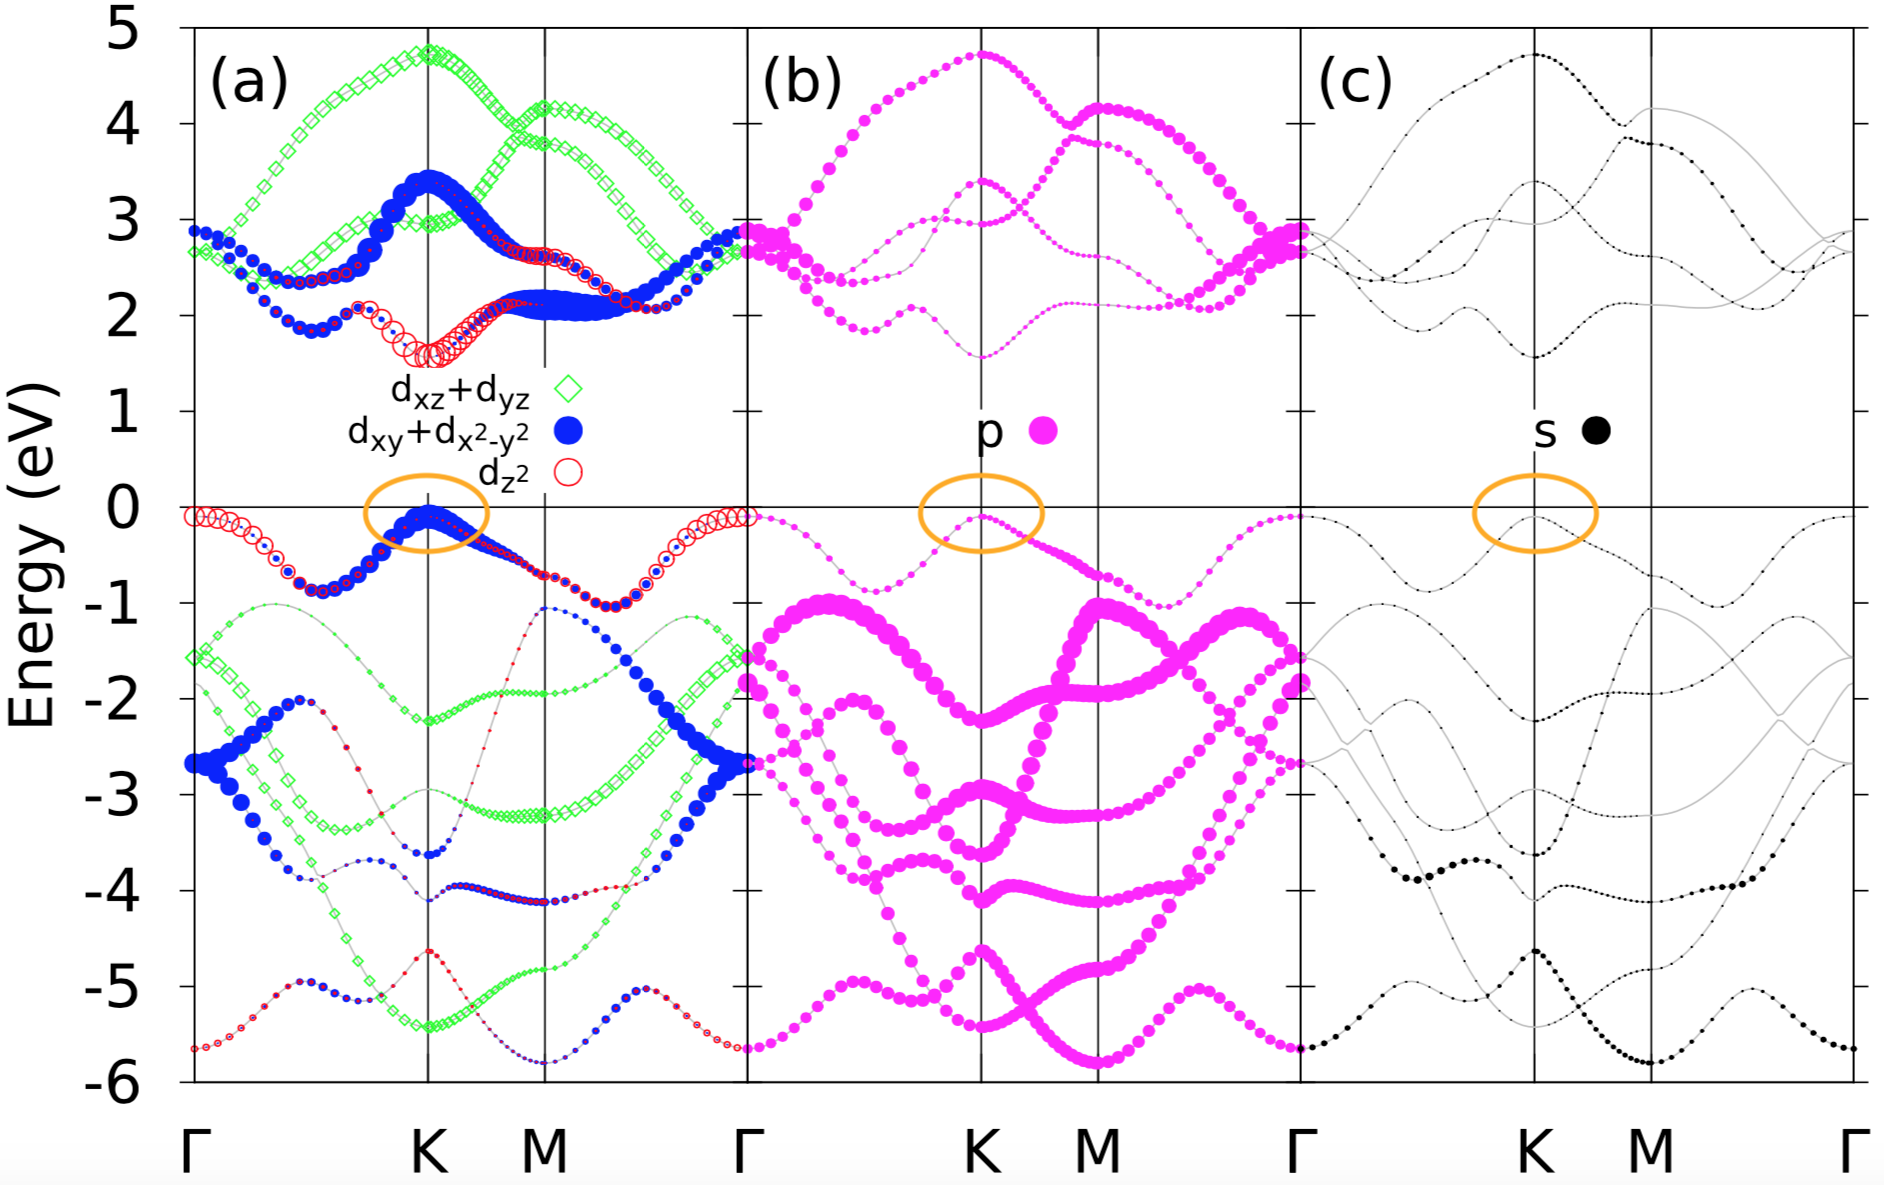
\includegraphics[width = 10cm]{Introduction/energiesTMDs}
\caption[Orbital projected band structures for monolayer $\text{Mo}\text{S}_2$ obtained from first principles.]{Orbital projected band structures for monolayer $\text{Mo}\text{S}_2$ obtained from first principles.
The Fermi energy is set to 0, and the symbol size is proportional to the population of the state.
The panels represent the contributions from: (a) $\text{Mo}$ $d$-orbitals; (b) All $p$-orbitals, dominated by $\text{S}$ atoms; (c) All $s$-orbitals. }
\label{fig:energiesTMDs}
\end{figure}	

By fitting to first principles results obtained from density functional theory for the materials' energy bands, we obtain the hopping parameters.
This procedure leads to a non-uniform nearest neighbor (NN) hopping matrix on the $M$-atom triangular lattice.
Since the argument is purely based on symmetry, in general, the $d-d$ hoppings include both direct $d-d$ interactions of $M$ atoms, and indirect ones, mediated by $X-p$ orbitals.
These $M$-$M$ hoppings suffice to describe the band-edge properties near the $\pm K$ valleys.
By including third nearest neighbor hoppings, one can reproduce the energy dispersion in  the entire first Brillouin zone.

We start by introducing the spinless model, and then generalize it to include spin-orbit coupling.
Let the greek indices represent orbital space, and, for now, ignore spin.
Then, the Hamiltonian reads

\begin{equation}
\mathcal{H} = \sum_{i, j} \sum_{\alpha, \beta} c_{i,\alpha}^\dagger t_{\alpha \beta} ( \bm R_i - \bm R_j ) c_{j, \beta}
\end{equation}

Considering the basis set $\{ d_{z^2} , d_{x y}, d_{ x^2 - y^2 } \} $, the on-site energies $\varepsilon_j$ corresponding to the atomic orbitals $\left| \phi_\mu^j \right\rangle$ appear through $\bm t ( \bm 0 ) = \text{diag} ( \varepsilon_1, \varepsilon_2, \varepsilon_2 )$, while the NN hoppings are (see Fig.(\ref{fig:tmdHex}))

\begin{equation}
\bm t ( \bm R_{1, 4} ) =
\begin{pmatrix}
t_0 & \pm t_1 & t_2 \\
\mp t_1 & t_{11} & \pm t_{12} \\
t_2 & \mp t_{12} & t_{22} \\
\end{pmatrix}
\end{equation}

\begin{equation}
\bm t (\, \bm R_{\substack{2, 5 \\ (3, 6)}} ) =
\begin{pmatrix}
t_0 & \Pm \bigg( \pm \frac{1}{2} t_1 - \frac{\sqrt{3}}{2} t_2 \bigg) & \mp \frac{\sqrt{3}}{2} t_1 - \frac{1}{2} t_2 \\
\Pm \bigg( \mp \frac{1}{2} t_1 - \frac{\sqrt{3}}{2} t_2 \bigg) & \frac{1}{4} ( t_{11} + 3 t_{22} ) & \Pm \bigg( \frac{\sqrt{3}}{4} ( t_{22} - t_{11} ) \mp t_{12} \bigg) \\
\pm \frac{\sqrt{3}}{2} t_1 - \frac{1}{2} t_2 & \Pm \bigg( \frac{\sqrt{3}}{4} ( t_{22} - t_{11} ) \pm t_{12} \bigg) & \frac{1}{4} ( 3 t_{11} + t_{22} )
\end{pmatrix}
\end{equation}